% Created by tikzDevice version 0.12.3.1 on 2020-07-05 15:32:10
% !TEX encoding = UTF-8 Unicode
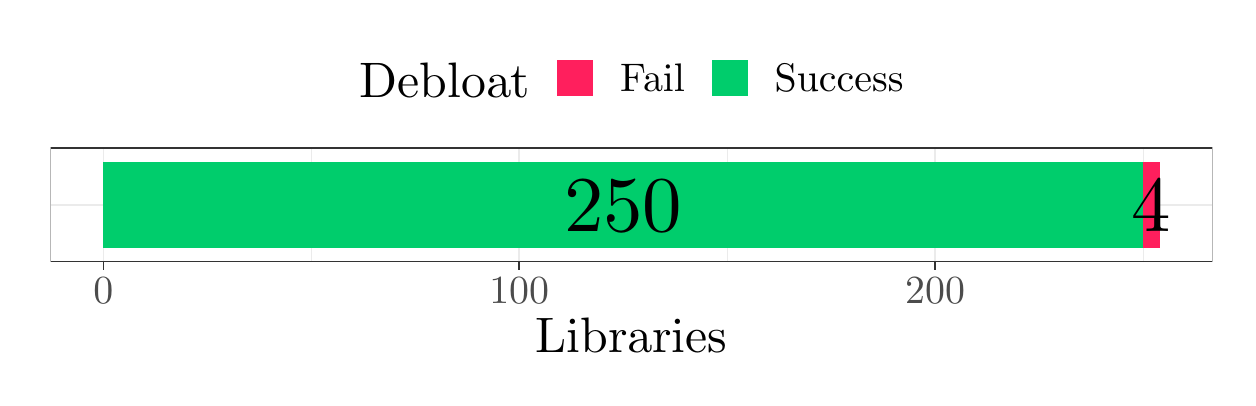
\begin{tikzpicture}[x=1pt,y=1pt]
\definecolor{fillColor}{RGB}{255,255,255}
\path[use as bounding box,fill=fillColor,fill opacity=0.00] (0,0) rectangle (433.62,126.47);
\begin{scope}
\path[clip] (  0.00,  0.00) rectangle (433.62,126.47);
\definecolor{drawColor}{RGB}{255,255,255}
\definecolor{fillColor}{RGB}{255,255,255}

\path[draw=drawColor,line width= 0.6pt,line join=round,line cap=round,fill=fillColor] (  0.00,  0.00) rectangle (433.62,126.47);
\end{scope}
\begin{scope}
\path[clip] (  8.25, 41.81) rectangle (428.12, 83.08);
\definecolor{fillColor}{RGB}{255,255,255}

\path[fill=fillColor] (  8.25, 41.81) rectangle (428.12, 83.08);
\definecolor{drawColor}{gray}{0.92}

\path[draw=drawColor,line width= 0.3pt,line join=round] (102.47, 41.81) --
	(102.47, 83.08);

\path[draw=drawColor,line width= 0.3pt,line join=round] (252.75, 41.81) --
	(252.75, 83.08);

\path[draw=drawColor,line width= 0.3pt,line join=round] (403.02, 41.81) --
	(403.02, 83.08);

\path[draw=drawColor,line width= 0.6pt,line join=round] (  8.25, 62.44) --
	(428.12, 62.44);

\path[draw=drawColor,line width= 0.6pt,line join=round] ( 27.34, 41.81) --
	( 27.34, 83.08);

\path[draw=drawColor,line width= 0.6pt,line join=round] (177.61, 41.81) --
	(177.61, 83.08);

\path[draw=drawColor,line width= 0.6pt,line join=round] (327.89, 41.81) --
	(327.89, 83.08);
\definecolor{fillColor}{RGB}{255,31,93}

\path[fill=fillColor] (403.02, 46.97) rectangle (409.04, 77.92);
\definecolor{fillColor}{RGB}{0,205,108}

\path[fill=fillColor] ( 27.34, 46.97) rectangle (403.02, 77.92);
\definecolor{drawColor}{RGB}{0,0,0}

\node[text=drawColor,anchor=base,inner sep=0pt, outer sep=0pt, scale=  2.85] at (406.03, 52.65) {4};

\node[text=drawColor,anchor=base,inner sep=0pt, outer sep=0pt, scale=  2.85] at (215.18, 52.65) {250};
\definecolor{drawColor}{gray}{0.20}

\path[draw=drawColor,line width= 0.6pt,line join=round,line cap=round] (  8.25, 41.81) rectangle (428.12, 83.08);
\end{scope}
\begin{scope}
\path[clip] (  0.00,  0.00) rectangle (433.62,126.47);
\definecolor{drawColor}{gray}{0.20}

\path[draw=drawColor,line width= 0.6pt,line join=round] ( 27.34, 39.06) --
	( 27.34, 41.81);

\path[draw=drawColor,line width= 0.6pt,line join=round] (177.61, 39.06) --
	(177.61, 41.81);

\path[draw=drawColor,line width= 0.6pt,line join=round] (327.89, 39.06) --
	(327.89, 41.81);
\end{scope}
\begin{scope}
\path[clip] (  0.00,  0.00) rectangle (433.62,126.47);
\definecolor{drawColor}{gray}{0.30}

\node[text=drawColor,anchor=base,inner sep=0pt, outer sep=0pt, scale=  1.44] at ( 27.34, 26.95) {0};

\node[text=drawColor,anchor=base,inner sep=0pt, outer sep=0pt, scale=  1.44] at (177.61, 26.95) {100};

\node[text=drawColor,anchor=base,inner sep=0pt, outer sep=0pt, scale=  1.44] at (327.89, 26.95) {200};
\end{scope}
\begin{scope}
\path[clip] (  0.00,  0.00) rectangle (433.62,126.47);
\definecolor{drawColor}{RGB}{0,0,0}

\node[text=drawColor,anchor=base,inner sep=0pt, outer sep=0pt, scale=  1.80] at (218.18,  9.00) {Libraries};
\end{scope}
\begin{scope}
\path[clip] (  0.00,  0.00) rectangle (433.62,126.47);
\definecolor{fillColor}{RGB}{255,255,255}

\path[fill=fillColor] (114.39, 94.08) rectangle (321.98,120.97);
\end{scope}
\begin{scope}
\path[clip] (  0.00,  0.00) rectangle (433.62,126.47);
\definecolor{drawColor}{RGB}{0,0,0}

\node[text=drawColor,anchor=base west,inner sep=0pt, outer sep=0pt, scale=  1.80] at (119.89,101.33) {Debloat};
\end{scope}
\begin{scope}
\path[clip] (  0.00,  0.00) rectangle (433.62,126.47);
\definecolor{fillColor}{RGB}{255,255,255}

\path[fill=fillColor] (190.63,101.02) rectangle (205.08,115.47);
\end{scope}
\begin{scope}
\path[clip] (  0.00,  0.00) rectangle (433.62,126.47);
\definecolor{fillColor}{RGB}{255,31,93}

\path[fill=fillColor] (191.34,101.73) rectangle (204.37,114.76);
\end{scope}
\begin{scope}
\path[clip] (  0.00,  0.00) rectangle (433.62,126.47);
\definecolor{fillColor}{RGB}{255,255,255}

\path[fill=fillColor] (246.48,101.02) rectangle (260.93,115.47);
\end{scope}
\begin{scope}
\path[clip] (  0.00,  0.00) rectangle (433.62,126.47);
\definecolor{fillColor}{RGB}{0,205,108}

\path[fill=fillColor] (247.19,101.73) rectangle (260.22,114.76);
\end{scope}
\begin{scope}
\path[clip] (  0.00,  0.00) rectangle (433.62,126.47);
\definecolor{drawColor}{RGB}{0,0,0}

\node[text=drawColor,anchor=base west,inner sep=0pt, outer sep=0pt, scale=  1.44] at (214.08,103.29) {Fail};
\end{scope}
\begin{scope}
\path[clip] (  0.00,  0.00) rectangle (433.62,126.47);
\definecolor{drawColor}{RGB}{0,0,0}

\node[text=drawColor,anchor=base west,inner sep=0pt, outer sep=0pt, scale=  1.44] at (269.93,103.29) {Success};
\end{scope}
\end{tikzpicture}
